% !TeX spellcheck = en_GB

% ------------------------------- %

\begin{frame}{\dots dataset}

\begin{columns}[T]
\begin{column}{0.5\textwidth}

\end{column}
\begin{column}{0.5\textwidth}
Binary classification task% (disease -- no disease)

Class distribution: 0:0.49 -- 1:0.51

Approaches
\begin{itemize}
	\item Decision tree
	\item Random forest
	\item AdaBoost
	\item Ridge logistic regression
	\item Super learner
\end{itemize}
\end{column}
\end{columns}

\end{frame}

% ------------------------------- %



% ------------------------------- %

\begin{frame}{What's a Super Learner?}

\begin{figure}
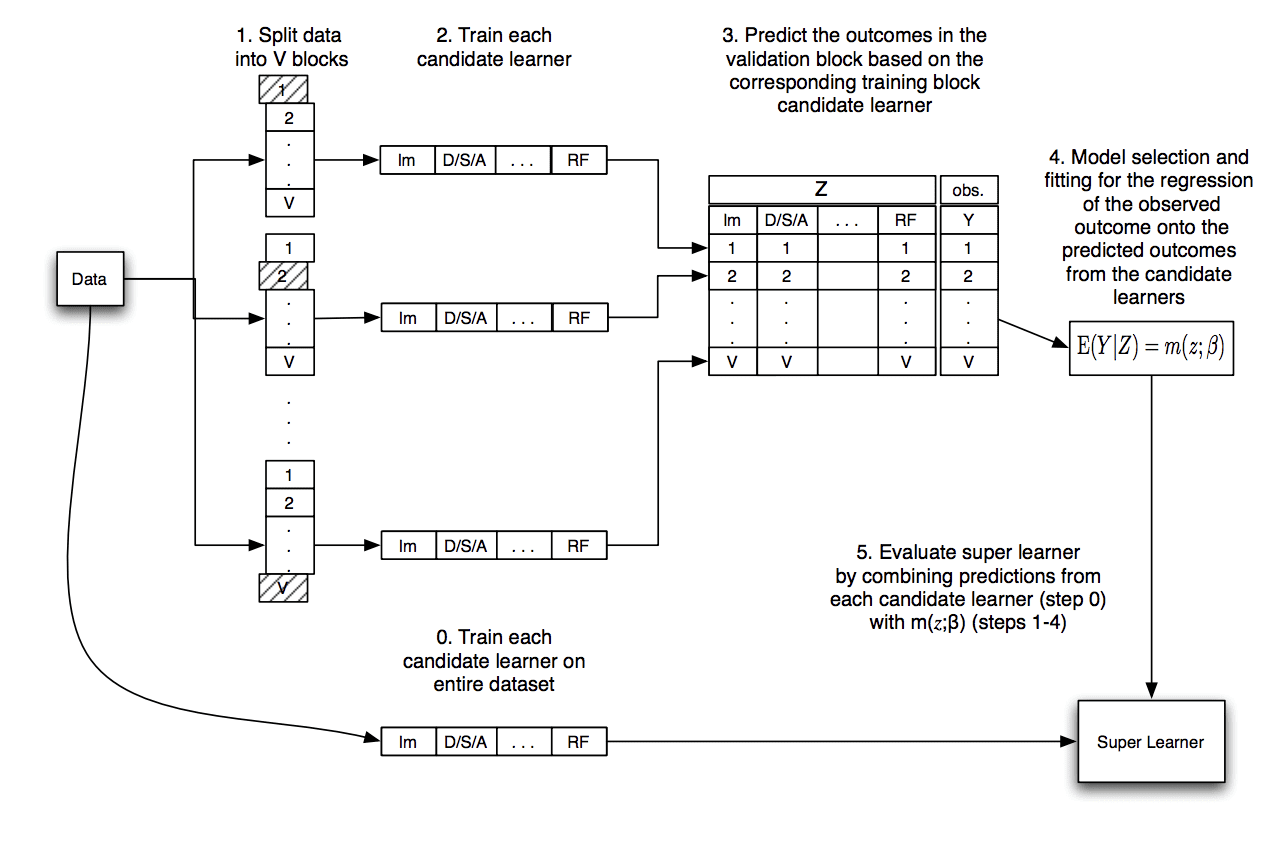
\includegraphics[width=\textwidth]{./Figures/sup-learn.jpg}
\end{figure}

\end{frame}

\begin{frame}{The Super Learner flow diagram}

\begin{tikzpicture}
	\tikzset{help lines/.append style=pink}
%	\draw [help lines] (-5,-4) grid (6,4); \node[draw,circle,red] at (0,0) {};

	% start with full training data
	\node[right,font=\small] (data) at (-5,0) {$\mathcal{D}=\set{(x_i,y_i)}_1^N$};

	% path 1: full training data
	\node[draw,rectangle,minimum width=2cm,minimum height=0.5cm,font=\small] (full) at (-1,2) {$\hat{\phi}_1, \hat{\phi}_2,\dots,\hat{\phi}_K$};
	\begingroup\linespread{0.9}\node[font=\footnotesize,text centered,text width=2.5cm] at ($(full)+(0,0.8)$) {strong learners on full $\mathcal{D}$, $\hat{\phi}_k(\boldsymbol{X})$};\endgroup
	\begingroup\linespread{0.9}\draw[-latex,bend left,thick] (data.north) to node[font=\footnotesize,above left,text centered,text width=1.5cm] {learners prediction} (full.west);\endgroup

	% path 2: cross-validation for weights
	\node[font=\footnotesize,below] (cross) at (0,-1.5) {
		$\begin{array}{cccc|c}
			\hat{\phi}_1 & \hat{\phi}_2 &\dots & \hat{\phi}_K & Y \\
			1 & 1 & \dots & 1 & 1 \\
			2 & 2 & \dots & 2 & 2 \\
			\vdots & \vdots & \ddots & \vdots & \vdots \\
			V & V & \dots & V & V
		\end{array}$
	};
	\begingroup\linespread{0.95}\node[font=\footnotesize,text centered,text width=3cm] at ($(cross.north)+(0,0.4)$) {cross-validation $\hat{\phi}_{k,T(\nu)}(\boldsymbol{X}_{V(\nu)})$};\endgroup
	\begingroup\linespread{0.9}\draw[-latex,thick,bend right] (data.south) to node[font=\footnotesize,below left,text centered,text width=1.5cm] {prediction weights} (cross);\endgroup

	% end with prediction
	\node[left] (pred) at (6,0) {$\hat{\phi}_{\text{SL}}=\sum_{k=1}^K{\color{mLightGreen}\hat{\alpha}_k}{\color{mLightBrown}\hat{\phi}_k}$};
	\draw[-latex,bend left,thick,mLightBrown] (full.east) to (pred);
%	\draw[-latex,thick,bend right,mLightGreen] (cross) to node[font=\scriptsize,below right,mDarkTeal] {$\argmin_\alpha\sum_{i=1}^NL(Y_i,m(z_i\rvert\alpha))$} (pred);
	\draw[-latex,thick,bend right,mLightGreen] (cross) to (pred);
	\node[font=\scriptsize] (alph) at (4,3.5) {$\hat{\alpha}=\argmin_\alpha\sum_{i=1}^NL(Y_i,m(z_i\rvert\alpha))$};
	\node[font=\scriptsize] at ($(alph)+(0,-0.55)$) {$m(z\rvert\alpha)=\sum_{k=1}^K\alpha_k\hat{\phi}_{k,T(\nu)}\bigl(\boldsymbol{X}_{V(\nu)}\bigr)$};
\end{tikzpicture}

\end{frame}

\begin{frame}{Super learner in practice}

Package \texttt{SuperLearner}

\end{frame}

% ------------------------------- %

\begin{frame}{Scores}

% il super learner riesce a prendere il meglio da questi modelli??

\begin{table}
\sisetup{round-mode=places}
\resizebox{0.9\textwidth}{!}{
\vspace*{-1em}\begin{tabular}{lS[round-precision=4]S[round-precision=4]}
\toprule
Model & {Train score} & {Test score} \\
\midrule
CART & 0. & 0. \\
Random forest & 0. & 0. \\
AdaBoost & 0. & 0. \\
Super learner & 0. & 0. \\
\bottomrule
\end{tabular}}
\end{table}

\end{frame}








